% Topic 4.5: Zero-Knowledge Technology in Finance [ADVANCED]
% Digital Finance Introduction
\documentclass[11pt,aspectratio=169]{beamer}
\usetheme{Madrid}

% ======================= PACKAGES =======================
\usepackage{graphicx}
\usepackage{booktabs}
\usepackage{adjustbox}
\usepackage{multicol}
\usepackage{amsmath}
\usepackage{amssymb}
\usepackage{tikz}
\usetikzlibrary{arrows,shapes,positioning,shadows,trees}
\usepackage{listings}
\usepackage{xcolor}

% ======================= COLOR DEFINITIONS =======================
% Primary color scheme: Blue/Teal for Digital Finance
\definecolor{dfblue}{RGB}{0,102,204}
\definecolor{dfteal}{RGB}{0,153,153}
\definecolor{dfcyan}{RGB}{51,187,204}
\definecolor{dflightblue}{RGB}{153,204,255}
\definecolor{dflightblue2}{RGB}{173,214,255}
\definecolor{dflightblue3}{RGB}{193,224,255}
\definecolor{dflightblue4}{RGB}{213,234,255}

% Accent colors for finance applications
\definecolor{dfgreen}{RGB}{44, 160, 44}
\definecolor{dfred}{RGB}{214, 39, 40}
\definecolor{dforange}{RGB}{255, 127, 14}
\definecolor{dfgray}{RGB}{127, 127, 127}

% Utility colors
\definecolor{lightgray}{RGB}{240, 240, 240}
\definecolor{midgray}{RGB}{180, 180, 180}
\definecolor{codebg}{RGB}{245, 245, 245}

% ======================= THEME CUSTOMIZATION =======================
% Apply Digital Finance color scheme to Madrid theme
\setbeamercolor{palette primary}{bg=dflightblue3,fg=dfblue}
\setbeamercolor{palette secondary}{bg=dflightblue2,fg=dfblue}
\setbeamercolor{palette tertiary}{bg=dfteal,fg=white}
\setbeamercolor{palette quaternary}{bg=dfblue,fg=white}

\setbeamercolor{structure}{fg=dfblue}
\setbeamercolor{section in toc}{fg=dfblue}
\setbeamercolor{subsection in toc}{fg=dfteal}
\setbeamercolor{title}{fg=dfblue}
\setbeamercolor{frametitle}{fg=dfblue,bg=dflightblue3}
\setbeamercolor{block title}{bg=dflightblue2,fg=dfblue}
\setbeamercolor{block body}{bg=dflightblue4,fg=black}

% Remove navigation symbols for cleaner look
\setbeamertemplate{navigation symbols}{}

% Clean itemize/enumerate
\setbeamertemplate{itemize items}[circle]
\setbeamertemplate{enumerate items}[default]

% Margins for readability
\setbeamersize{text margin left=8mm,text margin right=8mm}

% ======================= LISTINGS CONFIGURATION =======================
% Python code style
\lstdefinestyle{pythonstyle}{
    language=Python,
    basicstyle=\ttfamily\footnotesize,
    keywordstyle=\color{dfblue}\bfseries,
    stringstyle=\color{dforange},
    commentstyle=\color{dfgray}\itshape,
    numberstyle=\tiny\color{dfgray},
    numbers=left,
    numbersep=5pt,
    backgroundcolor=\color{codebg},
    showspaces=false,
    showstringspaces=false,
    showtabs=false,
    frame=single,
    rulecolor=\color{midgray},
    tabsize=4,
    captionpos=b,
    breaklines=true,
    breakatwhitespace=false,
    escapeinside={(*@}{@*)},
    xleftmargin=10pt,
    xrightmargin=10pt
}

% Solidity code style
\lstdefinestyle{soliditystyle}{
    language=Java, % closest approximation
    basicstyle=\ttfamily\footnotesize,
    keywordstyle=\color{dfteal}\bfseries,
    stringstyle=\color{dforange},
    commentstyle=\color{dfgray}\itshape,
    numberstyle=\tiny\color{dfgray},
    numbers=left,
    numbersep=5pt,
    backgroundcolor=\color{codebg},
    showspaces=false,
    showstringspaces=false,
    showtabs=false,
    frame=single,
    rulecolor=\color{midgray},
    tabsize=2,
    captionpos=b,
    breaklines=true,
    breakatwhitespace=false,
    escapeinside={(*@}{@*)},
    xleftmargin=10pt,
    xrightmargin=10pt,
    morekeywords={pragma, contract, function, returns, public, private, view, pure, payable, address, uint256, mapping, event, modifier}
}

% Inline code command
\newcommand{\code}[1]{\texttt{\color{dfblue}#1}}

% ======================= CUSTOM COMMANDS =======================
% Bottom annotation (Madrid-style)
\newcommand{\bottomnote}[1]{%
\vfill
\vspace{-2mm}
\textcolor{dflightblue2}{\rule{\textwidth}{0.4pt}}
\vspace{1mm}
\footnotesize
\textbf{#1}
}

% Compact list spacing
\newcommand{\compactlist}{%
\setlength{\itemsep}{0pt}%
\setlength{\parskip}{0pt}%
\setlength{\parsep}{0pt}%
}

% Chart placeholder
\newcommand{\chartplaceholder}[2][5cm]{%
\begin{center}
\begin{adjustbox}{max width=0.95\textwidth, max height=#1}
\framebox[\textwidth][c]{%
\rule{0pt}{#1}%
\textcolor{midgray}{[#2]}%
}
\end{adjustbox}
\end{center}
}

% ======================= FINANCE NOTATION MACROS =======================
% Probability and statistics
\newcommand{\E}{\mathbb{E}} % Expected value
\newcommand{\Var}{\mathrm{Var}} % Variance
\newcommand{\Cov}{\mathrm{Cov}} % Covariance
\newcommand{\Prob}{\mathbb{P}} % Probability

% Distributions
\newcommand{\Normal}{\mathcal{N}} % Normal distribution
\newcommand{\Uniform}{\mathcal{U}} % Uniform distribution

% Returns and prices
\newcommand{\Ret}{R} % Return
\newcommand{\LogRet}{r} % Log return
\newcommand{\Price}{S} % Price/Stock price
\newcommand{\Strike}{K} % Strike price

% Options and derivatives
\newcommand{\CallPrice}{C} % Call option price
\newcommand{\PutPrice}{P} % Put option price
\newcommand{\Greeks}[1]{\mathit{#1}} % Greek letters

% Risk measures
\newcommand{\VaR}{\mathrm{VaR}} % Value at Risk
\newcommand{\CVaR}{\mathrm{CVaR}} % Conditional VaR
\newcommand{\Sharpe}{\mathrm{SR}} % Sharpe Ratio

% Time series
\newcommand{\AR}{\mathrm{AR}} % Autoregressive
\newcommand{\MA}{\mathrm{MA}} % Moving average
\newcommand{\GARCH}{\mathrm{GARCH}} % GARCH

% Blockchain/Crypto
\newcommand{\Hash}{\mathrm{Hash}} % Hash function
\newcommand{\Block}{\mathcal{B}} % Block
\newcommand{\Chain}{\mathcal{C}} % Chain

% Real numbers, integers
\newcommand{\R}{\mathbb{R}}
\newcommand{\Z}{\mathbb{Z}}
\newcommand{\N}{\mathbb{N}}

% ======================= TIKZ STYLES =======================
% Styles for finance-related diagrams
\tikzstyle{process} = [rectangle, minimum width=3cm, minimum height=1cm, text centered, draw=dfblue, fill=dflightblue4, thick]
\tikzstyle{decision} = [diamond, minimum width=3cm, minimum height=1cm, text centered, draw=dfteal, fill=dflightblue4, thick]
\tikzstyle{arrow} = [thick,->,>=stealth,color=dfblue]
\tikzstyle{blockchain} = [rectangle, rounded corners, minimum width=2.5cm, minimum height=1cm, text centered, draw=dfteal, fill=dflightblue3, thick]
\tikzstyle{transaction} = [circle, minimum size=0.8cm, text centered, draw=dforange, fill=dflightblue4, thick]

% ======================= FOOTER TEMPLATE =======================
\setbeamertemplate{footline}{
    \hbox{\begin{beamercolorbox}[wd=\paperwidth,ht=2.5ex,dp=1ex,leftskip=.5em,rightskip=.5em]{author in head/foot}
    \tiny
    \textbf{Digital Finance} \hfill
    Joerg Osterrieder \hfill
    \insertdate \hfill
    Page \insertframenumber{} / \inserttotalframenumber
    \end{beamercolorbox}}
}

% ======================= SECTION DIVIDER TEMPLATE =======================
\AtBeginSection[]{
\begin{frame}[plain]
\vfill
\centering
\begin{beamercolorbox}[sep=12pt,center]{title}
\usebeamerfont{title}\LARGE\insertsection\par
\end{beamercolorbox}
\vfill
\end{frame}
}


% Additional packages for tables
\usepackage{multirow}

% Additional TikZ libraries for ZK diagrams
\usetikzlibrary{chains,calc,decorations.pathreplacing,fit,backgrounds}

% Custom styles (from T3.2)
\tikzstyle{blocknode} = [rectangle, rounded corners, minimum width=3cm, minimum height=2cm, text centered, draw=dfteal, fill=dflightblue3, thick]
\tikzstyle{hashbox} = [rectangle, rounded corners, minimum width=2cm, minimum height=0.8cm, text centered, draw=dfteal, fill=dflightblue3, thick, font=\footnotesize]
\tikzstyle{databox} = [rectangle, minimum width=2.5cm, minimum height=0.6cm, text centered, draw=dfblue, fill=dflightblue4, thick, font=\footnotesize]
\tikzstyle{keybox} = [rectangle, rounded corners, minimum width=2cm, minimum height=0.6cm, text centered, draw=dforange, fill=dflightblue4, thick, font=\footnotesize]
\tikzstyle{walletbox} = [rectangle, rounded corners, minimum width=2.5cm, minimum height=1cm, text centered, draw=dfgreen, fill=dflightblue4, thick]
\tikzstyle{networknode} = [circle, draw=dfblue, fill=dflightblue4, minimum size=0.8cm, thick]
% ZK-specific styles
\tikzstyle{proverbox} = [rectangle, rounded corners, minimum width=3cm, minimum height=1.2cm, text centered, draw=dfgreen, fill=dfgreen!15, thick]
\tikzstyle{verifierbox} = [rectangle, rounded corners, minimum width=3cm, minimum height=1.2cm, text centered, draw=dfblue, fill=dfblue!15, thick]
\tikzstyle{proofbox} = [rectangle, rounded corners, minimum width=2cm, minimum height=0.8cm, text centered, draw=dforange, fill=dforange!15, thick]
\tikzstyle{secretbox} = [rectangle, rounded corners, minimum width=2cm, minimum height=0.8cm, text centered, draw=dfred, fill=dfred!15, thick]
\tikzstyle{zkprotocol} = [rectangle, rounded corners, minimum width=2.5cm, minimum height=1cm, text centered, draw=dfpurple, fill=dfpurple!15, thick]

\title[Topic 4.5: Zero-Knowledge]{Topic 4.5: Zero-Knowledge Technology in Finance [ADVANCED]}
\subtitle{Privacy and Scalability Through Mathematical Proofs}
\author{Joerg Osterrieder}
\institute{Digital Finance}
\date{2025}

\begin{document}

% =======================================================================
% SLIDE 1: TITLE SLIDE
% =======================================================================
\begin{frame}[plain]
\titlepage
\end{frame}

% =======================================================================
% SLIDE 2: LEARNING OBJECTIVES
% =======================================================================
\begin{frame}{Learning Objectives}
\textbf{By the end of this topic, you will be able to:}

\begin{enumerate}
\item \textbf{Explain} what zero-knowledge proofs are and why they matter for finance
\vspace{2mm}
\item \textbf{Describe} the three essential properties: completeness (honest people succeed), soundness (liars get caught), and zero-knowledge (no secrets leaked)
\vspace{2mm}
\item \textbf{Compare} SNARKs (Succinct Non-interactive ARgument of Knowledge) and STARKs (Scalable Transparent ARgument of Knowledge) in terms of tradeoffs and use cases
\vspace{2mm}
\item \textbf{Identify} key applications of ZK technology in privacy, scaling, and identity
\vspace{2mm}
\item \textbf{Evaluate} the privacy-regulation tradeoff enabled by ZK proofs
\vspace{2mm}
\item \textbf{Assess} the implications of ZK technology for financial compliance
\end{enumerate}

\vspace{3mm}
\begin{block}{Core Question}
How can you prove you know something without revealing what you know?
\end{block}
\end{frame}

% =======================================================================
% SLIDE 3: PREREQUISITES - CRYPTOGRAPHY RECAP
% =======================================================================
\begin{frame}{Prerequisites: Cryptographic Foundations}
\textbf{From Topic 3.1 and 3.2 -- Key Concepts You'll Need:}

\begin{columns}[T]
\begin{column}{0.48\textwidth}
\textbf{Hash Functions}
\begin{itemize}\compactlist
\item One-way transformation
\item Deterministic output
\item Collision resistant
\item Used in commitments
\end{itemize}
\textit{Think: Digital fingerprint -- unique, can't be forged}

\vspace{3mm}
\textbf{Digital Signatures}
\begin{itemize}\compactlist
\item Private key signs
\item Public key verifies
\item Non-repudiation
\item Authentication
\end{itemize}
\textit{Think: Handwritten signature, but mathematically unforgeable}
\end{column}
\begin{column}{0.48\textwidth}
\textbf{Public Key Cryptography}
\begin{itemize}\compactlist
\item Asymmetric key pairs
\item Mathematical trapdoors
\item Encryption and signing
\item Foundation for ZK proofs
\end{itemize}
\textit{Think: Mailbox -- anyone can drop mail in (public key), only you can open it (private key)}

\vspace{3mm}
\textbf{Why This Matters:}
\begin{itemize}\compactlist
\item ZK proofs build on these primitives
\item Understanding foundations helps intuition
\item Same cryptographic assumptions
\end{itemize}
\end{column}
\end{columns}

\bottomnote{If these concepts are unfamiliar, review Topics 3.1-3.2 before continuing}
\end{frame}

% =======================================================================
% SLIDE 4: PREREQUISITES - L2 AND ROLLUPS RECAP
% =======================================================================
\begin{frame}{Prerequisites: Layer 2 and Rollups}
\textbf{What is Layer 2?} Solutions built on top of Ethereum to make it faster and cheaper while inheriting its security.

\vspace{2mm}
\textbf{From Topic 3.2 -- Scaling Context:}

\begin{center}
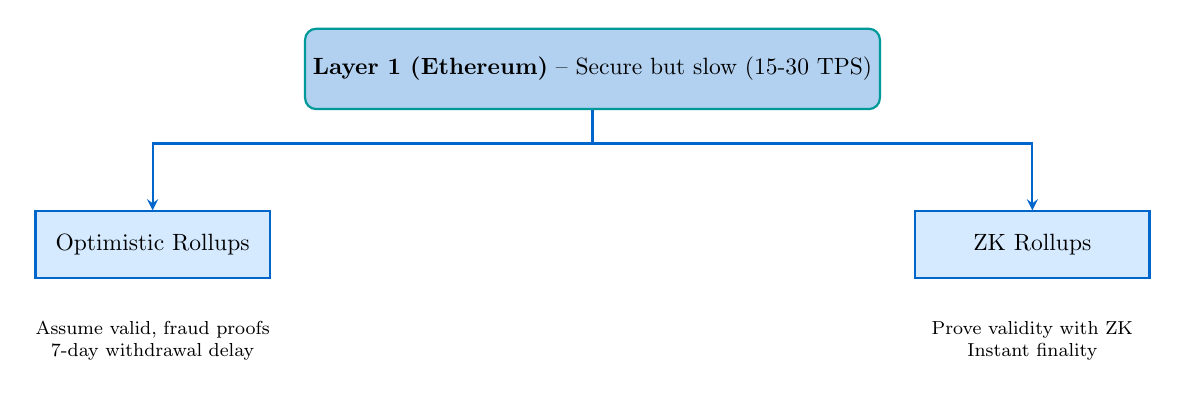
\begin{tikzpicture}[node distance=0.5cm, scale=0.85, transform shape]
% L1
\node[blocknode, minimum width=8cm, minimum height=1.2cm, fill=dfblue!30] (l1) {
\textbf{Layer 1 (Ethereum)} -- Secure but slow (15-30 TPS)
};

% L2 solutions
\node[process, minimum width=3.5cm, below left=1.5cm and 0.5cm of l1] (opt) {Optimistic Rollups};
\node[process, minimum width=3.5cm, below right=1.5cm and 0.5cm of l1] (zk) {ZK Rollups};

% Characteristics
\node[below=0.5cm of opt, font=\footnotesize, text width=3.5cm, align=center] {
Assume valid, fraud proofs\\
7-day withdrawal delay
};
\node[below=0.5cm of zk, font=\footnotesize, text width=3.5cm, align=center] {
Prove validity with ZK\\
Instant finality
};

\draw[arrow] (l1.south) -- ++(0,-0.5) -| (opt.north);
\draw[arrow] (l1.south) -- ++(0,-0.5) -| (zk.north);
\end{tikzpicture}
\end{center}

\vspace{3mm}
\textbf{Today's Focus:} Understanding the ``ZK'' in ZK-Rollups

\begin{block}{Key Insight}
Zero-knowledge proofs enable trustless verification: instead of trusting someone's claim, you can mathematically verify it's true.
\end{block}
\end{frame}

% =======================================================================
% SLIDE 5: WHAT IS ZERO-KNOWLEDGE?
% =======================================================================
\begin{frame}{What is Zero-Knowledge?}
\begin{center}
\textit{``A zero-knowledge proof lets you prove you know something,\\without revealing what that something is.''}
\end{center}

\vspace{5mm}
\begin{columns}[T]
\begin{column}{0.48\textwidth}
\textbf{Traditional Proof}
\begin{itemize}\compactlist
\item ``I know the password''
\item $\rightarrow$ Type the password
\item Verifier sees the secret
\item Password is now exposed
\end{itemize}
\end{column}
\begin{column}{0.48\textwidth}
\textbf{Zero-Knowledge Proof}
\begin{itemize}\compactlist
\item ``I know the password''
\item $\rightarrow$ Prove via cryptographic protocol
\item Verifier is convinced
\item Password stays secret
\end{itemize}
\end{column}
\end{columns}

\vspace{3mm}
\textbf{How?} The prover demonstrates knowledge by responding to random challenges that only someone with the secret could answer correctly -- but the answers themselves don't reveal the secret.

\vspace{3mm}
\begin{block}{Formal Definition}
A \textbf{zero-knowledge proof} is a method by which a \textit{prover} can convince a \textit{verifier} that a statement is true, without conveying any information apart from the fact that the statement is indeed true.
\end{block}
\end{frame}

% =======================================================================
% SLIDE 6: COLORBLIND FRIEND ANALOGY - SETUP
% =======================================================================
\begin{frame}{The Colorblind Friend Analogy (Part 1)}
\textbf{The Classic ZK Explanation:}

\begin{columns}[T]
\begin{column}{0.55\textwidth}
\textbf{The Setup:}
\begin{itemize}
\item You have two balls: one \textcolor{dfred}{RED}, one \textcolor{dfgreen}{GREEN}
\item Your friend is colorblind -- they look identical to him
\item He claims: ``These balls are the same color''
\item You want to \textbf{prove} they're different
\item But you don't want to reveal \textbf{which is which}
\end{itemize}

\vspace{3mm}
\textbf{Why This is a ZK Problem:}
\begin{itemize}
\item \textbf{Statement:} ``I can distinguish these balls''
\item \textbf{Secret:} Which color is which
\item \textbf{Goal:} Convince friend without teaching him colors
\end{itemize}
\end{column}
\begin{column}{0.42\textwidth}
\begin{center}
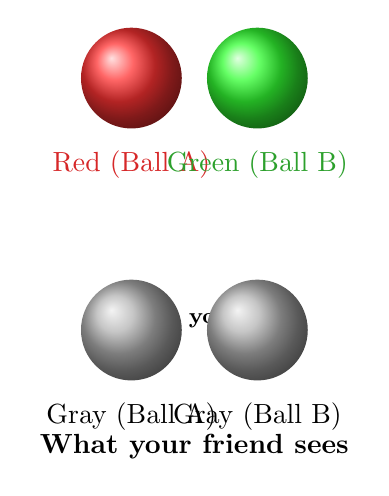
\begin{tikzpicture}[scale=0.8]
% Two balls
\shade[ball color=red!80] (-1, 0) circle (0.8);
\shade[ball color=green!80] (1, 0) circle (0.8);

% Labels
\node[below] at (-1, -1) {\textcolor{dfred}{Red (Ball A)}};
\node[below] at (1, -1) {\textcolor{dfgreen}{Green (Ball B)}};

% Friend view
\node[below=2cm, text width=4cm, align=center, font=\footnotesize] at (0, -1) {
\textbf{What you see}
};

\shade[ball color=gray!60] (-1, -4) circle (0.8);
\shade[ball color=gray!60] (1, -4) circle (0.8);
\node[below] at (-1, -5) {Gray (Ball A)};
\node[below] at (1, -5) {Gray (Ball B)};
\node[below] at (0, -5.5) {\textbf{What your friend sees}};
\end{tikzpicture}
\end{center}
\end{column}
\end{columns}
\end{frame}

% =======================================================================
% SLIDE 7: COLORBLIND FRIEND ANALOGY - PROTOCOL
% =======================================================================
\begin{frame}{The Colorblind Friend Analogy (Part 2)}
\textbf{The Protocol:}

\begin{center}
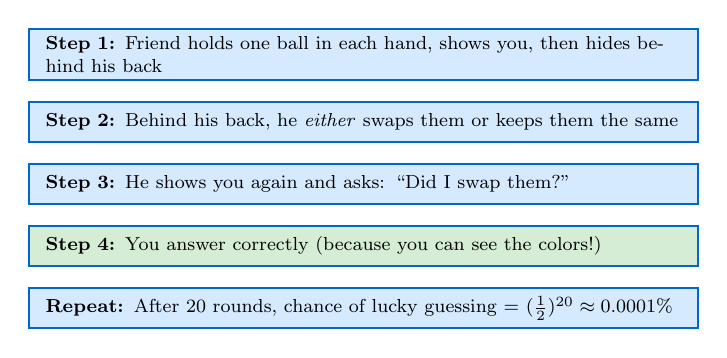
\begin{tikzpicture}[node distance=0.3cm, scale=0.85, transform shape]
% Steps
\node[databox, minimum width=10cm, text width=9.5cm, align=left] (s1) {
\textbf{Step 1:} Friend holds one ball in each hand, shows you, then hides behind his back
};
\node[databox, minimum width=10cm, text width=9.5cm, align=left, below=0.3cm of s1] (s2) {
\textbf{Step 2:} Behind his back, he \textit{either} swaps them or keeps them the same
};
\node[databox, minimum width=10cm, text width=9.5cm, align=left, below=0.3cm of s2] (s3) {
\textbf{Step 3:} He shows you again and asks: ``Did I swap them?''
};
\node[databox, minimum width=10cm, text width=9.5cm, align=left, below=0.3cm of s3, fill=dfgreen!20] (s4) {
\textbf{Step 4:} You answer correctly (because you can see the colors!)
};
\node[databox, minimum width=10cm, text width=9.5cm, align=left, below=0.3cm of s4] (s5) {
\textbf{Repeat:} After 20 rounds, chance of lucky guessing = $(\frac{1}{2})^{20} \approx 0.0001\%$
};
\end{tikzpicture}
\end{center}

\vspace{3mm}
\begin{block}{The Zero-Knowledge Property}
Your friend becomes convinced the balls are different colors, but learns \textbf{nothing} about which ball is red and which is green. You could run this protocol a million times and he still couldn't learn the colors.
\end{block}
\end{frame}

% =======================================================================
% SLIDE 8: THREE PROPERTIES OF ZK PROOFS
% =======================================================================
\begin{frame}{The Three Essential Properties}
\textbf{Every zero-knowledge proof must satisfy these three properties:}

\vspace{3mm}
\begin{block}{In Plain English}
\textbf{Completeness} = honest people succeed. \textbf{Soundness} = liars get caught. \textbf{Zero-Knowledge} = no secrets leaked.
\end{block}

\vspace{3mm}
\begin{columns}[T]
\begin{column}{0.32\textwidth}
\begin{center}
\textbf{\textcolor{dfgreen}{1. Completeness}}
\end{center}
\begin{itemize}\compactlist
\item If the statement is \textbf{true}
\item And prover is \textbf{honest}
\item Verifier will be \textbf{convinced}
\end{itemize}

\vspace{3mm}
\textit{``True claims succeed''}
\end{column}
\begin{column}{0.32\textwidth}
\begin{center}
\textbf{\textcolor{dfred}{2. Soundness}}
\end{center}
\begin{itemize}\compactlist
\item If the statement is \textbf{false}
\item No cheating prover can convince the verifier
\item (Except with tiny probability)
\end{itemize}

\vspace{3mm}
\textit{``False claims fail''}
\end{column}
\begin{column}{0.32\textwidth}
\begin{center}
\textbf{\textcolor{dfblue}{3. Zero-Knowledge}}
\end{center}
\begin{itemize}\compactlist
\item Verifier learns \textbf{nothing}
\item Except that statement is true
\item Could simulate proof alone
\end{itemize}

\vspace{3mm}
\textit{``No info leaked''}
\end{column}
\end{columns}

\vspace{3mm}
\begin{center}
\fbox{\parbox{0.75\textwidth}{\centering
\textbf{All three are required.} Missing any one breaks the system:\\
No completeness = useless. No soundness = insecure. No zero-knowledge = not private.
}}
\end{center}
\end{frame}

% =======================================================================
% SLIDE 9: PROPERTIES ILLUSTRATED
% =======================================================================
\begin{frame}{The Three Properties Illustrated}
\textbf{Back to the Colorblind Friend:}

\begin{center}
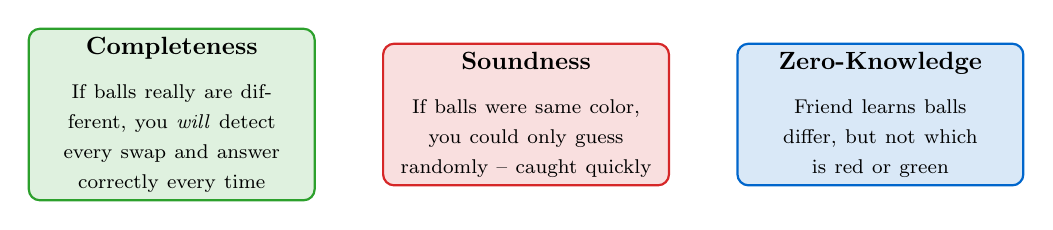
\begin{tikzpicture}[node distance=0.5cm, scale=0.9, transform shape]
% Completeness
\node[proverbox, minimum width=4cm, text width=3.8cm, align=center] (c) at (-5, 0) {
\textbf{Completeness}\\[2mm]
\footnotesize If balls really are different, you \textit{will} detect every swap and answer correctly every time
};

% Soundness
\node[secretbox, minimum width=4cm, text width=3.8cm, align=center] (s) at (0, 0) {
\textbf{Soundness}\\[2mm]
\footnotesize If balls were same color, you could only guess randomly -- caught quickly
};

% Zero-Knowledge
\node[verifierbox, minimum width=4cm, text width=3.8cm, align=center] (z) at (5, 0) {
\textbf{Zero-Knowledge}\\[2mm]
\footnotesize Friend learns balls differ, but not which is red or green
};
\end{tikzpicture}
\end{center}

\vspace{5mm}
\textbf{Mathematical Interpretation:}
\begin{itemize}
\item \textbf{Completeness:} The chance that a true statement is accepted is 100\%. Notation: $\Pr[\text{Verifier accepts} | \text{statement true}] = 1$
\item \textbf{Soundness:} The chance that a false statement is accepted is negligible (essentially zero). Notation: $\Pr[\text{Verifier accepts} | \text{statement false}] \leq \epsilon$
\item \textbf{Zero-Knowledge:} Verifier's view can be simulated without the secret
\end{itemize}
\end{frame}

% =======================================================================
% SLIDE 10: INTERACTIVE VS NON-INTERACTIVE
% =======================================================================
\begin{frame}{Interactive vs. Non-Interactive Proofs}
\begin{columns}[T]
\begin{column}{0.48\textwidth}
\textbf{Interactive Proofs}

\begin{center}
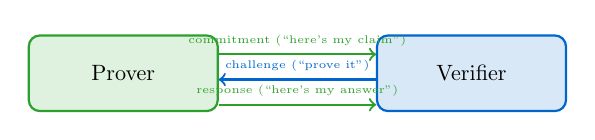
\begin{tikzpicture}[node distance=0.4cm, scale=0.8, transform shape]
\node[proverbox] (p) {Prover};
\node[verifierbox, right=2.5cm of p] (v) {Verifier};

\draw[->, thick, dfgreen] ([yshift=0.3cm]p.east) -- node[above, font=\tiny] {commitment (``here's my claim'')} ([yshift=0.3cm]v.west);
\draw[->, thick, dfblue] ([yshift=-0.1cm]v.west) -- node[above, font=\tiny] {challenge (``prove it'')} ([yshift=-0.1cm]p.east);
\draw[->, thick, dfgreen] ([yshift=-0.5cm]p.east) -- node[above, font=\tiny] {response (``here's my answer'')} ([yshift=-0.5cm]v.west);
\end{tikzpicture}
\end{center}

\vspace{3mm}
\begin{itemize}\compactlist
\item Multiple rounds of communication
\item Verifier sends random challenges
\item Prover responds to each challenge
\item Like the colorblind friend example
\end{itemize}

\textcolor{dfred}{Problem: Requires both parties online}
\end{column}
\begin{column}{0.48\textwidth}
\textbf{Non-Interactive Proofs}

\begin{center}
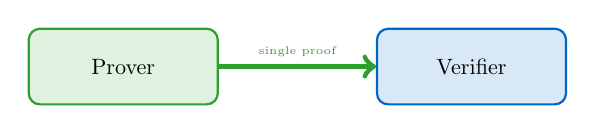
\begin{tikzpicture}[node distance=0.4cm, scale=0.8, transform shape]
\node[proverbox] (p) {Prover};
\node[verifierbox, right=2.5cm of p] (v) {Verifier};

\draw[->, thick, dfgreen, line width=2pt] (p.east) -- node[above, font=\tiny] {single proof} (v.west);
\end{tikzpicture}
\end{center}

\vspace{3mm}
\begin{itemize}\compactlist
\item Single message from prover
\item No back-and-forth required
\item Proof can be verified anytime
\item Essential for blockchain use
\end{itemize}

\textcolor{dfgreen}{Solution: Fiat-Shamir transform}
\end{column}
\end{columns}

\vspace{3mm}
\begin{block}{Key Insight}
The \textbf{Fiat-Shamir heuristic} converts interactive proofs to non-interactive by using a hash function to generate ``random'' challenges deterministically. This enables ZK proofs on blockchains.
\end{block}
\end{frame}

% =======================================================================
% SLIDE 11: FIAT-SHAMIR TRANSFORM
% =======================================================================
\begin{frame}{The Fiat-Shamir Transform}
\textbf{How to Remove Interaction:}

\begin{center}
\begin{tikzpicture}[node distance=0.5cm, scale=0.85, transform shape]
% Interactive
\node[font=\bfseries] at (-4.5, 3) {Interactive};
\node[proverbox, minimum width=2.5cm] (p1) at (-6, 1.5) {Prover};
\node[verifierbox, minimum width=2.5cm] (v1) at (-3, 1.5) {Verifier};

\draw[->, thick] ([yshift=0.2cm]p1.east) -- node[above, font=\tiny] {commit} ([yshift=0.2cm]v1.west);
\draw[->, thick, dfred] (v1.west) -- node[below, font=\tiny] {random r} (p1.east);
\draw[->, thick] ([yshift=-0.4cm]p1.east) -- node[below, font=\tiny] {response} ([yshift=-0.4cm]v1.west);

% Arrow
\draw[->, ultra thick, dfpurple] (-0.5, 1.5) -- node[above] {Fiat-Shamir} (1.5, 1.5);

% Non-interactive
\node[font=\bfseries] at (4.5, 3) {Non-Interactive};
\node[proverbox, minimum width=2.5cm] (p2) at (3, 1.5) {Prover};
\node[verifierbox, minimum width=2.5cm] (v2) at (6, 1.5) {Verifier};

\draw[->, ultra thick, dfgreen] (p2.east) -- node[above, font=\tiny] {proof $\pi$} (v2.west);

% Hash explanation
\node[hashbox, minimum width=4cm, below=1.5cm of p2, text width=3.8cm, align=center] (hash) {
$r = \text{Hash}(\text{commit})$\\
\footnotesize Deterministic ``randomness''
};
\draw[->, thick, dashed] (hash.north) -- (p2.south);
\end{tikzpicture}
\end{center}

\vspace{3mm}
\textbf{The Trick:} Instead of waiting for verifier's random challenge, the prover:
\begin{enumerate}
\item Computes the commitment
\item Hashes the commitment to get a ``random'' challenge
\item Computes the response
\item Packages everything into a single proof
\end{enumerate}
\end{frame}

% =======================================================================
% SLIDE 12: SNARKs INTUITION
% =======================================================================
\begin{frame}{SNARKs: Succinct Non-Interactive Arguments of Knowledge}
\textbf{What does SNARK stand for?}

\vspace{2mm}
\textit{Think of SNARK and STARK as two different recipes for making the same meal -- both create zero-knowledge proofs, just with different ingredients and tradeoffs.}

\vspace{3mm}
\begin{center}
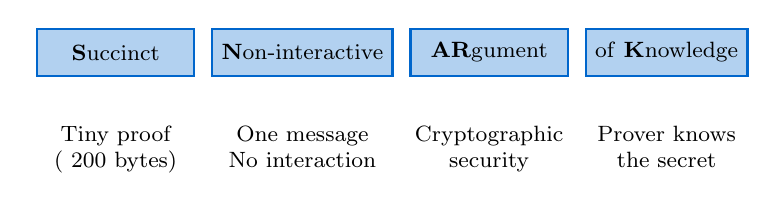
\begin{tikzpicture}[node distance=0.3cm]
\node[databox, minimum width=2cm, fill=dfblue!30] (s) {\textbf{S}uccinct};
\node[databox, minimum width=2cm, fill=dfblue!30, right=0.2cm of s] (n) {\textbf{N}on-interactive};
\node[databox, minimum width=2cm, fill=dfblue!30, right=0.2cm of n] (a) {\textbf{AR}gument};
\node[databox, minimum width=2cm, fill=dfblue!30, right=0.2cm of a] (k) {of \textbf{K}nowledge};

\node[below=0.5cm of s, font=\footnotesize, text width=2cm, align=center] {Tiny proof\\(~200 bytes)};
\node[below=0.5cm of n, font=\footnotesize, text width=2cm, align=center] {One message\\No interaction};
\node[below=0.5cm of a, font=\footnotesize, text width=2cm, align=center] {Cryptographic\\security};
\node[below=0.5cm of k, font=\footnotesize, text width=2cm, align=center] {Prover knows\\the secret};
\end{tikzpicture}
\end{center}

\vspace{5mm}
\begin{columns}[T]
\begin{column}{0.48\textwidth}
\textbf{Key Properties:}
\begin{itemize}\compactlist
\item \textbf{Tiny proofs:} ~200 bytes regardless of computation size
\item \textbf{Fast verification:} Milliseconds
\item \textbf{One-time setup:} Trusted setup ceremony
\end{itemize}
\end{column}
\begin{column}{0.48\textwidth}
\textbf{The Catch -- Trusted Setup:}
\begin{itemize}\compactlist
\item Requires generating ``toxic waste''
\item If anyone keeps the waste, they can forge proofs
\item Multi-party ceremonies distribute trust
\end{itemize}
\end{column}
\end{columns}
\end{frame}

% =======================================================================
% SLIDE 13: SNARKs - TRUSTED SETUP
% =======================================================================
\begin{frame}{SNARKs: The Trusted Setup Problem}
\textbf{What is a Trusted Setup?}

\begin{center}
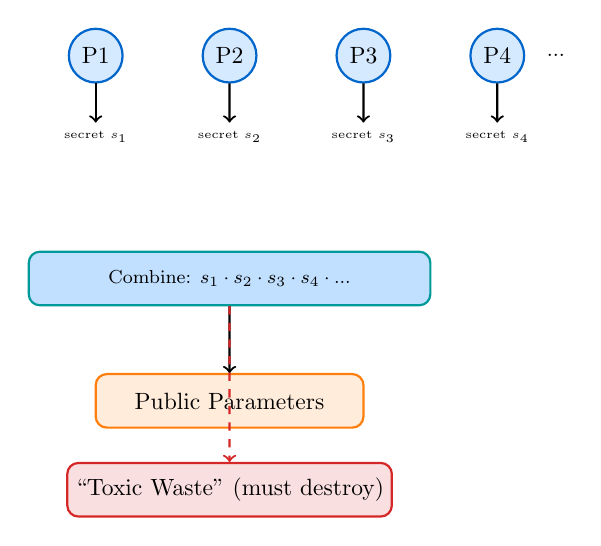
\begin{tikzpicture}[node distance=0.5cm, scale=0.85, transform shape]
% Ceremony participants
\node[networknode] (p1) at (0, 2) {P1};
\node[networknode] (p2) at (2, 2) {P2};
\node[networknode] (p3) at (4, 2) {P3};
\node[networknode] (p4) at (6, 2) {P4};
\node[right=0.2cm of p4, font=\small] {...};

% Generate secrets
\draw[->, thick] (p1) -- ++(0, -1) node[below, font=\tiny] {secret $s_1$};
\draw[->, thick] (p2) -- ++(0, -1) node[below, font=\tiny] {secret $s_2$};
\draw[->, thick] (p3) -- ++(0, -1) node[below, font=\tiny] {secret $s_3$};
\draw[->, thick] (p4) -- ++(0, -1) node[below, font=\tiny] {secret $s_4$};

% Combine
\node[hashbox, minimum width=6cm, below=2.5cm of p2] (combine) {Combine: $s_1 \cdot s_2 \cdot s_3 \cdot s_4 \cdot ...$};

% Output
\node[proofbox, below=1cm of combine, minimum width=4cm] (params) {Public Parameters};
\node[secretbox, below=0.5cm of params, minimum width=4cm] (toxic) {``Toxic Waste'' (must destroy)};

\draw[->, thick] (combine) -- (params);
\draw[->, thick, dashed, dfred] (combine) -- (toxic);
\end{tikzpicture}
\end{center}

\vspace{2mm}
\textbf{Security Assumption:} At least ONE participant must honestly destroy their secret. If all secrets combine and are destroyed, the system is secure.

\bottomnote{Zcash's Powers of Tau ceremony had 87 participants; zkSync's had thousands}
\end{frame}

% =======================================================================
% SLIDE 14: STARKs INTUITION
% =======================================================================
\begin{frame}{STARKs: Scalable Transparent Arguments of Knowledge}
\textbf{What does STARK stand for?}

\vspace{2mm}
\textit{STARK = the same meal as SNARK, but using publicly available ingredients (no secret recipe required).}

\vspace{3mm}
\begin{center}
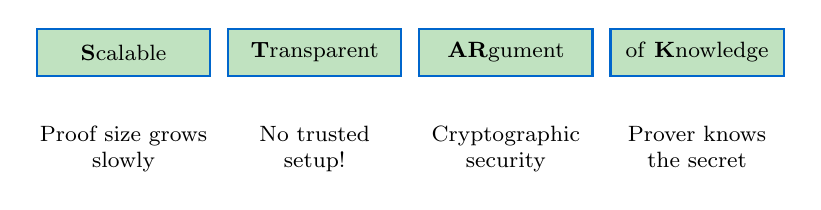
\begin{tikzpicture}[node distance=0.3cm]
\node[databox, minimum width=2.2cm, fill=dfgreen!30] (s) {\textbf{S}calable};
\node[databox, minimum width=2.2cm, fill=dfgreen!30, right=0.2cm of s] (t) {\textbf{T}ransparent};
\node[databox, minimum width=2.2cm, fill=dfgreen!30, right=0.2cm of t] (a) {\textbf{AR}gument};
\node[databox, minimum width=2.2cm, fill=dfgreen!30, right=0.2cm of a] (k) {of \textbf{K}nowledge};

\node[below=0.5cm of s, font=\footnotesize, text width=2.2cm, align=center] {Proof size grows\\slowly};
\node[below=0.5cm of t, font=\footnotesize, text width=2.2cm, align=center] {No trusted\\setup!};
\node[below=0.5cm of a, font=\footnotesize, text width=2.2cm, align=center] {Cryptographic\\security};
\node[below=0.5cm of k, font=\footnotesize, text width=2.2cm, align=center] {Prover knows\\the secret};
\end{tikzpicture}
\end{center}

\vspace{5mm}
\begin{columns}[T]
\begin{column}{0.48\textwidth}
\textbf{Advantages:}
\begin{itemize}\compactlist
\item \textcolor{dfgreen}{\textbf{No trusted setup}} -- Transparent
\item \textcolor{dfgreen}{\textbf{Quantum resistant}} -- Uses hash functions
\item \textcolor{dfgreen}{\textbf{Scalable proving}} -- Faster for large computations
\end{itemize}
\end{column}
\begin{column}{0.48\textwidth}
\textbf{Tradeoffs:}
\begin{itemize}\compactlist
\item \textcolor{dfred}{Larger proofs} -- ~50KB vs ~200 bytes
\item \textcolor{dfred}{Newer technology} -- Less battle-tested
\item Still fast verification
\end{itemize}
\end{column}
\end{columns}
\end{frame}

% =======================================================================
% SLIDE 15: STARKs - HOW TRANSPARENCY WORKS
% =======================================================================
\begin{frame}{STARKs: Achieving Transparency}
\textbf{How do STARKs avoid trusted setup?}

\begin{columns}[T]
\begin{column}{0.55\textwidth}
\textbf{The Key Difference:}
\begin{itemize}
\item SNARKs use \textbf{elliptic curves} -- require special parameters
\item STARKs use only \textbf{hash functions} -- publicly known, no secrets needed
\end{itemize}

\vspace{3mm}
\textbf{Why Hash Functions?}
\begin{itemize}\compactlist
\item SHA-256, Poseidon, etc. are standardized
\item No hidden trapdoors
\item Anyone can verify the math
\item Quantum computers can't break them (easily)
\end{itemize}

\vspace{3mm}
\textbf{The Tradeoff:}\\
Transparency costs proof size. Hash-based cryptography produces larger proofs than elliptic curve cryptography.
\end{column}
\begin{column}{0.42\textwidth}
\begin{center}
\begin{tikzpicture}[scale=0.8]
% SNARK
\node[zkprotocol, minimum width=3.5cm, minimum height=2cm, text width=3.3cm, align=center] (snark) at (0, 2) {
\textbf{SNARK}\\[2mm]
\footnotesize Elliptic curves\\
Trusted setup
};

% STARK
\node[zkprotocol, minimum width=3.5cm, minimum height=2cm, text width=3.3cm, align=center, fill=dfgreen!20] (stark) at (0, -1) {
\textbf{STARK}\\[2mm]
\footnotesize Hash functions\\
Transparent
};

\draw[->, ultra thick] (snark) -- node[right, font=\footnotesize] {Remove trust} (stark);
\end{tikzpicture}
\end{center}
\end{column}
\end{columns}
\end{frame}

% =======================================================================
% SLIDE 16: SNARK VS STARK COMPARISON
% =======================================================================
\begin{frame}{SNARK vs. STARK: Head-to-Head Comparison}
\begin{center}
\begin{tabular}{l|c|c}
\toprule
\textbf{Property} & \textbf{SNARK} & \textbf{STARK} \\
\midrule
Proof Size & \textcolor{dfgreen}{~200 bytes (tiny)} & \textcolor{dfred}{~50 KB (larger)} \\
Verification Time & Fast (milliseconds) & Fast (milliseconds) \\
Prover Time & Moderate & Faster for large computations \\
\midrule
Trusted Setup & \textcolor{dfred}{Required (ceremony)} & \textcolor{dfgreen}{Not required (transparent)} \\
Quantum Resistant & \textcolor{dfred}{No} & \textcolor{dfgreen}{Yes (hash-based)} \\
\midrule
Maturity & Battle-tested since 2016 & Newer (2018+) \\
\midrule
Examples & Zcash, zkSync Era & StarkNet, StarkEx \\
 & Polygon zkEVM & dYdX, ImmutableX \\
\bottomrule
\end{tabular}
\end{center}

\vspace{5mm}
\begin{block}{Key Takeaway}
\textbf{SNARKs} win on proof size (important for on-chain verification costs).\\
\textbf{STARKs} win on trust assumptions and future-proofing against quantum computers.
\end{block}
\end{frame}

% =======================================================================
% SLIDE 17: ZK IN PRIVACY - OVERVIEW
% =======================================================================
\begin{frame}{ZK in Privacy: Hiding Transaction Details}
\textbf{The Problem with Public Blockchains:}

\begin{columns}[T]
\begin{column}{0.48\textwidth}
\textbf{Bitcoin/Ethereum Today:}
\begin{itemize}\compactlist
\item All transactions are public
\item Anyone can trace funds
\item Link addresses to identities
\item Complete financial surveillance
\end{itemize}

\vspace{3mm}
\textit{Would you want your bank statement public?}
\end{column}
\begin{column}{0.48\textwidth}
\textbf{With ZK Privacy:}
\begin{itemize}\compactlist
\item Transactions are encrypted
\item ZK proves validity without revealing details
\item Amount, sender, receiver hidden
\item Only authorized parties see data
\end{itemize}

\vspace{3mm}
\textit{Prove you paid without showing how much}
\end{column}
\end{columns}

\vspace{5mm}
\begin{center}
\begin{tikzpicture}[node distance=0.5cm]
\node[databox, minimum width=4cm, fill=dfred!20] (pub) {Public: Alice sent 5 ETH to Bob};
\node[databox, minimum width=4cm, fill=dfgreen!20, right=2cm of pub] (priv) {Private: Valid transaction occurred};

\draw[->, ultra thick, dfpurple] (pub) -- node[above, font=\small] {ZK} (priv);
\end{tikzpicture}
\end{center}
\end{frame}

% =======================================================================
% SLIDE 18: ZK IN PRIVACY - SHIELDED TRANSACTIONS
% =======================================================================
\begin{frame}{ZK in Privacy: Shielded Transactions}
\textbf{How Zcash Shielded Pools Work:}

\begin{center}
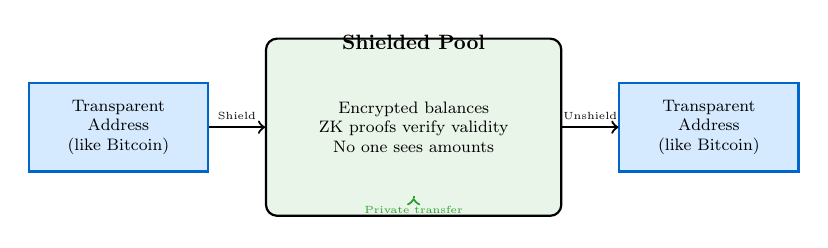
\begin{tikzpicture}[node distance=0.5cm, scale=0.75, transform shape]
% Transparent zone
\node[databox, minimum width=3cm, minimum height=1.5cm, fill=dflightblue4] (t1) at (-5, 0) {
\begin{minipage}{2.8cm}\centering
\footnotesize Transparent\\Address\\(like Bitcoin)
\end{minipage}
};

% Shielded pool
\node[draw, thick, rounded corners, minimum width=5cm, minimum height=3cm, fill=dfgreen!10] (pool) at (0, 0) {};
\node[above] at (0, 1.2) {\textbf{Shielded Pool}};
\node[font=\footnotesize, text width=4.5cm, align=center] at (0, 0) {
Encrypted balances\\
ZK proofs verify validity\\
No one sees amounts
};

% Another transparent
\node[databox, minimum width=3cm, minimum height=1.5cm, fill=dflightblue4] (t2) at (5, 0) {
\begin{minipage}{2.8cm}\centering
\footnotesize Transparent\\Address\\(like Bitcoin)
\end{minipage}
};

% Arrows
\draw[->, thick] (t1) -- node[above, font=\tiny] {Shield} (pool);
\draw[->, thick] (pool) -- node[above, font=\tiny] {Unshield} (t2);
\draw[->, thick, dfgreen] (0, -1.2) to[bend right=30] node[below, font=\tiny] {Private transfer} (0, -1.2);
\end{tikzpicture}
\end{center}

\vspace{3mm}
\textbf{What the ZK Proof Shows (Without Revealing):}
\begin{itemize}
\item The sender has sufficient balance (without showing the balance)
\item No double-spending occurred (without showing transaction history)
\item The amounts balance (inputs = outputs, without showing amounts)
\end{itemize}

\bottomnote{Zcash launched in 2016 -- first production ZK-SNARK system}
\end{frame}

% =======================================================================
% SLIDE 19: ZK IN SCALING - ZK ROLLUPS
% =======================================================================
\begin{frame}{ZK in Scaling: ZK-Rollups}
\textbf{How ZK Proofs Enable Scaling:}

\begin{center}
\begin{tikzpicture}[node distance=0.5cm, scale=0.8, transform shape]
% L2 transactions
\node[font=\bfseries] at (-5, 2.5) {Layer 2 (Off-chain)};
\node[databox, minimum width=1.5cm] (tx1) at (-6, 1.5) {Tx 1};
\node[databox, minimum width=1.5cm] (tx2) at (-5, 1.5) {Tx 2};
\node[databox, minimum width=1.5cm] (tx3) at (-4, 1.5) {Tx 3};
\node[right=0.1cm of tx3, font=\small] {...1000s};

% Rollup
\node[zkprotocol, minimum width=3.5cm, below=1cm of tx2, text width=3.3cm, align=center] (rollup) {
\textbf{ZK-Rollup}\\[1mm]
\footnotesize Batch + Generate proof
};

% L1
\node[font=\bfseries] at (4, 2.5) {Layer 1 (On-chain)};
\node[blocknode, minimum width=4cm, minimum height=2cm, text width=3.8cm, align=center] (l1) at (4, 0.5) {
\textbf{Ethereum}\\[2mm]
\footnotesize Verify ZK proof\\
Store state root\\
~200 byte proof
};

% Arrows
\draw[->, thick] (tx1) -- (rollup);
\draw[->, thick] (tx2) -- (rollup);
\draw[->, thick] (tx3) -- (rollup);
\draw[->, ultra thick, dfgreen] (rollup) -- node[above, font=\footnotesize] {Single proof} (l1);
\end{tikzpicture}
\end{center}

\vspace{2mm}
\textbf{The Magic:}
\begin{itemize}
\item 1000 transactions $\rightarrow$ 1 tiny proof (~200 bytes)
\item L1 verifies proof in milliseconds
\item Cost shared across all transactions
\item \textbf{Result:} 100x+ cheaper transactions with L1 security
\end{itemize}
\end{frame}

% =======================================================================
% SLIDE 20: ZK IN SCALING - VERIFICATION FLOW
% =======================================================================
\begin{frame}{ZK-Rollup Verification Flow}
\textbf{Step-by-step process:}

\begin{center}
\begin{tikzpicture}[node distance=0.8cm, scale=0.75, transform shape]
% Steps
\node[proverbox, minimum width=3.5cm, text width=3.3cm, align=center] (s1) {
\textbf{1. Collect}\\
\footnotesize Batch user transactions
};
\node[proverbox, minimum width=3.5cm, text width=3.3cm, align=center, right=0.5cm of s1] (s2) {
\textbf{2. Execute}\\
\footnotesize Process all txs off-chain
};
\node[zkprotocol, minimum width=3.5cm, text width=3.3cm, align=center, right=0.5cm of s2] (s3) {
\textbf{3. Prove}\\
\footnotesize Generate ZK proof
};

\node[verifierbox, minimum width=3.5cm, text width=3.3cm, align=center, below=1.5cm of s1] (s4) {
\textbf{4. Submit}\\
\footnotesize Post proof to L1
};
\node[verifierbox, minimum width=3.5cm, text width=3.3cm, align=center, right=0.5cm of s4] (s5) {
\textbf{5. Verify}\\
\footnotesize L1 contract checks proof
};
\node[blocknode, minimum width=3.5cm, minimum height=1.2cm, text width=3.3cm, align=center, right=0.5cm of s5, fill=dfgreen!30] (s6) {
\textbf{6. Finalize}\\
\footnotesize State updated, instant finality
};

\draw[->, thick] (s1) -- (s2);
\draw[->, thick] (s2) -- (s3);
\draw[->, thick] (s3) -- ++(0, -0.8) -| (s4);
\draw[->, thick] (s4) -- (s5);
\draw[->, thick] (s5) -- (s6);
\end{tikzpicture}
\end{center}

\vspace{5mm}
\begin{columns}[T]
\begin{column}{0.48\textwidth}
\textbf{Key Advantage over Optimistic Rollups:}
\begin{itemize}\compactlist
\item No 7-day withdrawal delay
\item Instant finality on L1
\item Mathematical certainty, not assumptions
\end{itemize}
\end{column}
\begin{column}{0.48\textwidth}
\textbf{Live ZK-Rollups:}
\begin{itemize}\compactlist
\item zkSync Era
\item Polygon zkEVM
\item StarkNet
\item Linea, Scroll
\end{itemize}
\end{column}
\end{columns}
\end{frame}

% =======================================================================
% SLIDE 21: ZK IN IDENTITY - SELECTIVE DISCLOSURE
% =======================================================================
\begin{frame}{ZK in Identity: Selective Disclosure}
\textbf{The Problem:} Proving attributes without revealing everything

\begin{center}
\begin{tikzpicture}[node distance=0.5cm, scale=0.85, transform shape]
% Traditional
\node[font=\bfseries] at (-4.5, 2.5) {Traditional};
\node[secretbox, minimum width=4cm, text width=3.8cm, align=left, font=\footnotesize] (trad) at (-4.5, 0.5) {
\textbf{ID Card Shows:}\\
Name: Alice Smith\\
DOB: Jan 15, 1995\\
Address: 123 Main St\\
ID\#: 123-45-6789\\
Photo, signature...
};

\node[below=0.3cm of trad, font=\footnotesize, text width=4cm, align=center, text=dfred] {
Bartender learns everything just to verify age
};

% Arrow
\draw[->, ultra thick, dfpurple] (-2, 0.5) -- node[above] {ZK} (0.5, 0.5);

% ZK version
\node[font=\bfseries] at (3.5, 2.5) {With ZK Proof};
\node[proverbox, minimum width=4cm, text width=3.8cm, align=center, font=\footnotesize] (zk) at (3.5, 0.5) {
\textbf{ZK Proof Shows:}\\[2mm]
``I am over 21''\\[2mm]
\textit{(nothing else)}
};

\node[below=0.3cm of zk, font=\footnotesize, text width=4cm, align=center, text=dfgreen] {
Bartender learns only what they need
};
\end{tikzpicture}
\end{center}

\vspace{3mm}
\begin{block}{Applications}
\begin{itemize}\compactlist
\item Age verification without revealing birthdate
\item Income proof without showing bank statements
\item Nationality verification without passport details
\item Credential verification without identity exposure
\end{itemize}
\end{block}
\end{frame}

% =======================================================================
% SLIDE 22: ZK IN IDENTITY - AGE VERIFICATION EXAMPLE
% =======================================================================
\begin{frame}{ZK Age Verification: How It Works}
\textbf{Step-by-step example:}

\begin{center}
\begin{tikzpicture}[node distance=0.5cm, scale=0.8, transform shape]
% Government issues credential
\node[blocknode, minimum width=3cm, minimum height=1.2cm, fill=dfblue!30] (gov) at (-5, 2) {Government};
\node[secretbox, minimum width=4cm, text width=3.8cm, align=center, below=0.8cm of gov, font=\footnotesize] (cred) {
\textbf{Signed Credential}\\
DOB: 1995-01-15\\
Gov signature
};

% User
\node[proverbox, minimum width=2.5cm] (user) at (0, 0) {Alice};

% Verifier
\node[verifierbox, minimum width=2.5cm] (bar) at (5, 0) {Bar};

% Flows
\draw[->, thick] (gov) -- (cred);
\draw[->, thick] (cred) -- node[left, font=\tiny] {stores} (user);

% ZK proof generation
\node[zkprotocol, minimum width=3.5cm, text width=3.3cm, align=center, below=1.5cm of user, font=\footnotesize] (zkgen) {
\textbf{Generate ZK Proof}\\
Input: DOB, Gov signature\\
Output: ``Age $\geq$ 21''
};

\draw[->, thick] (user) -- (zkgen);
\draw[->, ultra thick, dfgreen] (zkgen) -| node[below, pos=0.3, font=\tiny] {ZK proof only} (bar);

% What bar learns
\node[below=0.5cm of bar, font=\footnotesize, text width=3cm, align=center, text=dfgreen] {
Bar learns:\\
\checkmark\ Age $\geq$ 21\\
\checkmark\ Gov verified\\
Nothing else!
};
\end{tikzpicture}
\end{center}

\bottomnote{Projects: Polygon ID, Worldcoin, zkPass, Sismo}
\end{frame}

% =======================================================================
% SLIDE 23: ZK IN DEFI - PRIVATE AMMS
% =======================================================================
\begin{frame}{ZK in DeFi: Privacy-Preserving Protocols}
\textbf{Current DeFi Problem:}

\begin{columns}[T]
\begin{column}{0.48\textwidth}
\textbf{Public DeFi Today:}
\begin{itemize}\compactlist
\item All trades visible on-chain
\item MEV bots front-run transactions
\item Whale movements tracked
\item Trading strategies exposed
\end{itemize}

\vspace{3mm}
\textbf{ZK-Enabled DeFi:}
\begin{itemize}\compactlist
\item Trade privately
\item Prove solvency without showing balance
\item Compliant privacy (selective disclosure)
\item Protected trading strategies
\end{itemize}
\end{column}
\begin{column}{0.48\textwidth}
\begin{center}
\begin{tikzpicture}[scale=0.75]
% Private AMM
\node[pool, minimum width=3.5cm, minimum height=2cm, fill=dfgreen!20] (amm) {
\begin{minipage}{3cm}\centering
\textbf{Private AMM}\\[2mm]
\footnotesize Encrypted orders\\
ZK settlement
\end{minipage}
};

% Traders
\node[walletbox, minimum width=1.5cm, above left=1cm and 0.5cm of amm] (t1) {Trader};
\node[walletbox, minimum width=1.5cm, above right=1cm and 0.5cm of amm] (t2) {Trader};

\draw[->, thick, dashed] (t1) -- node[left, font=\tiny] {encrypted} (amm);
\draw[->, thick, dashed] (t2) -- node[right, font=\tiny] {encrypted} (amm);

% Public output
\node[databox, below=1cm of amm, minimum width=3cm, fill=dfblue!20] (out) {
\footnotesize Public: ``Trade occurred''
};
\draw[->, thick] (amm) -- (out);
\end{tikzpicture}
\end{center}
\end{column}
\end{columns}

\vspace{3mm}
\begin{block}{Examples}
Penumbra (private DEX), Railgun (private DeFi), Aztec (private L2 for DeFi)
\end{block}
\end{frame}

% =======================================================================
% SLIDE 24: ZK IN DEFI - COMPLIANT PRIVACY
% =======================================================================
\begin{frame}{ZK in DeFi: Compliant Privacy}
\textbf{The Regulatory Challenge:}

\begin{center}
\textit{``How can we have financial privacy without enabling crime?''}
\end{center}

\vspace{3mm}
\begin{columns}[T]
\begin{column}{0.48\textwidth}
\textbf{ZK-Enabled Compliance:}
\begin{itemize}
\item Prove funds are NOT from sanctioned addresses
\item Prove tax compliance without revealing income
\item Prove accredited investor status privately
\item Selective disclosure to regulators
\end{itemize}

\vspace{3mm}
\textbf{Key Insight:}\\
ZK proofs can prove \textit{absence} of problems (not on sanctions list) while maintaining privacy.
\end{column}
\begin{column}{0.48\textwidth}
\begin{center}
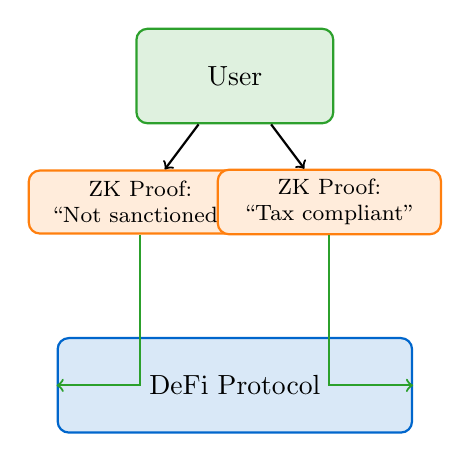
\begin{tikzpicture}[scale=0.8]
% User
\node[proverbox, minimum width=2.5cm] (user) at (0, 2) {User};

% Two proofs
\node[proofbox, minimum width=2.8cm, text width=2.6cm, align=center, font=\footnotesize] (p1) at (-1.5, 0) {
ZK Proof:\\
``Not sanctioned''
};
\node[proofbox, minimum width=2.8cm, text width=2.6cm, align=center, font=\footnotesize] (p2) at (1.5, 0) {
ZK Proof:\\
``Tax compliant''
};

% Protocol
\node[verifierbox, minimum width=4.5cm, below=1.2cm of user, yshift=-1.5cm] (proto) {DeFi Protocol};

\draw[->, thick] (user) -- (p1);
\draw[->, thick] (user) -- (p2);
\draw[->, thick, dfgreen] (p1) |- (proto);
\draw[->, thick, dfgreen] (p2) |- (proto);
\end{tikzpicture}
\end{center}
\end{column}
\end{columns}

\bottomnote{This approach is being explored for CBDC privacy as well (T4.4)}
\end{frame}

% =======================================================================
% SLIDE 25: HANDS-ON INTRODUCTION - NB16 PREVIEW
% =======================================================================
\begin{frame}{Hands-On: Introduction to ZK Concepts (NB16)}
\textbf{In the notebook, you will explore:}

\begin{enumerate}
\item \textbf{Hash Commitments} -- The building block of ZK
\vspace{2mm}
\item \textbf{Simple ZK Protocol} -- Prove you know a number without revealing it
\vspace{2mm}
\item \textbf{Range Proofs} -- Prove a value is in a range (like age $\geq$ 21)
\vspace{2mm}
\item \textbf{Merkle Proofs} -- Prove membership without revealing the set
\end{enumerate}

\vspace{5mm}
\begin{center}
\fbox{\parbox{0.8\textwidth}{\centering
\textbf{Learning Goal:} Develop intuition for how ZK proofs work by implementing simple versions of the core concepts.
}}
\end{center}

\vspace{3mm}
\textbf{Note:} Production ZK systems (SNARKs/STARKs) are much more complex, but the intuition from these exercises transfers directly.

\bottomnote{Open NB16\_zero\_knowledge\_intro.ipynb in Google Colab}
\end{frame}

% =======================================================================
% SLIDE 26: HANDS-ON - WHAT TO EXPECT
% =======================================================================
\begin{frame}[fragile]{NB16: What You'll Build}
\begin{columns}[T]
\begin{column}{0.55\textwidth}
\textbf{Exercise 1: Hash Commitment}
\begin{lstlisting}[style=pythonstyle, basicstyle=\ttfamily\tiny]
# Commit to a secret
secret = "my_password"
commitment = hash(secret + random_nonce)
# Later: reveal secret + nonce
# Verifier: hash(secret + nonce) == commitment?
\end{lstlisting}

\vspace{2mm}
\textbf{Exercise 2: Simple ZK Proof}
\begin{lstlisting}[style=pythonstyle, basicstyle=\ttfamily\tiny]
# Prove you know x where hash(x) = H
# Without revealing x
# Interactive: challenge-response protocol
\end{lstlisting}

\vspace{2mm}
\textbf{Exercise 3: Range Proof}
\begin{lstlisting}[style=pythonstyle, basicstyle=\ttfamily\tiny]
# Prove: 18 <= age <= 100
# Without revealing exact age
# Uses bit decomposition + commitments
\end{lstlisting}
\end{column}
\begin{column}{0.42\textwidth}
\begin{center}
\fbox{\parbox{0.95\textwidth}{
\textbf{Key Observations:}\\[2mm]
\footnotesize
1. Commitments hide data until reveal\\[1mm]
2. Challenges ensure prover isn't cheating\\[1mm]
3. Hash functions are the workhorse\\[1mm]
4. Randomness is essential for ZK property
}}
\end{center}

\vspace{3mm}
\textbf{Time estimate:} 45-60 minutes

\textbf{Prerequisites:} Python, basic understanding of hash functions

\vspace{3mm}
\textbf{Libraries used:}
\begin{itemize}\compactlist
\item \texttt{hashlib} (hashing)
\item \texttt{secrets} (randomness)
\end{itemize}
\end{column}
\end{columns}
\end{frame}

% =======================================================================
% SLIDE 27: DISCUSSION - PRIVACY VS REGULATION
% =======================================================================
\begin{frame}{Discussion: Privacy vs. Regulation}
\textbf{The Fundamental Tension:}

\begin{columns}[T]
\begin{column}{0.48\textwidth}
\textbf{Case for Privacy:}
\begin{itemize}\compactlist
\item Financial privacy is a human right
\item Surveillance chills legitimate activity
\item Protects against discrimination
\item Personal safety (wealth exposure)
\item Competitive business interests
\end{itemize}

\vspace{3mm}
\textit{``If you have nothing to hide, you have nothing to fear'' is a surveillance state argument}
\end{column}
\begin{column}{0.48\textwidth}
\textbf{Case for Transparency:}
\begin{itemize}\compactlist
\item Prevents money laundering
\item Tax compliance enforcement
\item Sanctions effectiveness
\item Counter-terrorism financing
\item Consumer protection
\end{itemize}

\vspace{3mm}
\textit{``Complete privacy enables crime without consequence''}
\end{column}
\end{columns}

\vspace{3mm}
\begin{block}{Discussion Questions}
\begin{itemize}
\item Can ZK proofs thread the needle between these positions?
\item Who decides what needs to be disclosed?
\item Is ``compliant privacy'' an oxymoron or a solution?
\end{itemize}
\end{block}
\end{frame}

% =======================================================================
% SLIDE 28: DISCUSSION - TORNADO CASH CASE
% =======================================================================
\begin{frame}{Discussion: The Tornado Cash Case Study}
\textbf{What Happened:}

\begin{columns}[T]
\begin{column}{0.55\textwidth}
\begin{itemize}
\item Tornado Cash: Ethereum privacy mixer
\item Used ZK proofs to break transaction links
\item August 2022: US Treasury sanctions
\item Developer arrested in Netherlands
\item Smart contract code itself sanctioned
\end{itemize}

\vspace{3mm}
\textbf{The Debate:}
\begin{itemize}\compactlist
\item Is code speech? (First Amendment)
\item Can open-source tools be sanctioned?
\item Developer liability for user actions?
\item Privacy tool vs. money laundering tool?
\end{itemize}
\end{column}
\begin{column}{0.42\textwidth}
\begin{alertblock}{Key Statistics}
\begin{itemize}\compactlist
\item \$7B+ total volume
\item ~30\% allegedly illicit (Chainalysis)
\item ~70\% legitimate privacy use
\item Still operational (code is immutable)
\end{itemize}
\end{alertblock}

\vspace{3mm}
\textbf{Implications:}
\begin{itemize}\compactlist
\item Chilling effect on privacy development
\item Precedent for sanctioning code
\item Push toward compliant privacy solutions
\end{itemize}
\end{column}
\end{columns}
\end{frame}

% =======================================================================
% SLIDE 29: DISCUSSION - FUTURE OF ZK PRIVACY
% =======================================================================
\begin{frame}{Discussion: The Future of ZK Privacy}
\textbf{Where are we heading?}

\begin{columns}[T]
\begin{column}{0.48\textwidth}
\textbf{Possible Scenarios:}

\textbf{1. Compliant Privacy Wins}
\begin{itemize}\compactlist
\item ZK proofs with selective disclosure
\item Regulators get access when needed
\item Privacy by default, transparency by exception
\end{itemize}

\vspace{2mm}
\textbf{2. Privacy Tech Restricted}
\begin{itemize}\compactlist
\item Heavy regulation of privacy tools
\item KYC required for all crypto
\item Privacy coins delisted
\end{itemize}
\end{column}
\begin{column}{0.48\textwidth}
\textbf{3. Parallel Systems}
\begin{itemize}\compactlist
\item Regulated ``light'' and unregulated ``dark'' finance
\item Similar to offshore banking today
\item Cat-and-mouse enforcement
\end{itemize}

\vspace{2mm}
\textbf{4. ZK Becomes Standard}
\begin{itemize}\compactlist
\item All transactions private by default
\item New compliance paradigms emerge
\item Privacy seen as security feature
\end{itemize}
\end{column}
\end{columns}

\vspace{3mm}
\begin{block}{Key Question}
Can we design systems where users have privacy, but bad actors can be identified? ZK proofs make this technically possible -- the question is governance.
\end{block}
\end{frame}

% =======================================================================
% SLIDE 30: EXECUTIVE SUMMARY
% =======================================================================
\begin{frame}{Executive Summary: Key Takeaways}
\begin{enumerate}
\item \textbf{Zero-knowledge proofs prove knowledge without revealing it}\\
Enable privacy-preserving verification through cryptographic magic.

\vspace{3mm}
\item \textbf{Three essential properties: Completeness, Soundness, Zero-Knowledge}\\
True claims succeed, false claims fail, no information leaks.

\vspace{3mm}
\item \textbf{SNARKs vs. STARKs trade off proof size for trust assumptions}\\
SNARKs: tiny proofs, trusted setup. STARKs: larger proofs, transparent.

\vspace{3mm}
\item \textbf{Applications span privacy, scaling, and identity}\\
Private transactions, ZK-rollups, and selective disclosure of credentials.

\vspace{3mm}
\item \textbf{ZK enables ``compliant privacy'' -- a potential middle ground}\\
Prove you're not a criminal without revealing your financial details.
\end{enumerate}
\end{frame}

% =======================================================================
% SLIDE 31: CONCEPT MAP
% =======================================================================
\begin{frame}{Concept Map: The ZK Ecosystem}
\begin{center}
\begin{tikzpicture}[scale=0.7, transform shape, node distance=1cm]
% Central node
\node[zkprotocol, minimum width=3cm, minimum height=1.2cm, fill=dfpurple!30] (zk) {\textbf{Zero-Knowledge}};

% Main branches
\node[proverbox, minimum width=2.5cm, above left=1.5cm and 1cm of zk] (tech) {Technology};
\node[verifierbox, minimum width=2.5cm, above right=1.5cm and 1cm of zk] (apps) {Applications};
\node[proofbox, minimum width=2.5cm, below=2cm of zk] (props) {Properties};

% Tech sub-nodes
\node[databox, above left=0.8cm and 0cm of tech, font=\scriptsize] (snark) {SNARKs};
\node[databox, above right=0.8cm and 0cm of tech, font=\scriptsize] (stark) {STARKs};

% Apps sub-nodes
\node[databox, above left=0.8cm and -0.5cm of apps, font=\scriptsize] (priv) {Privacy};
\node[databox, above=0.8cm of apps, font=\scriptsize] (scale) {Scaling};
\node[databox, above right=0.8cm and -0.5cm of apps, font=\scriptsize] (id) {Identity};

% Props sub-nodes
\node[databox, below left=0.5cm and 0cm of props, font=\scriptsize] (comp) {Complete};
\node[databox, below=0.5cm of props, font=\scriptsize] (sound) {Sound};
\node[databox, below right=0.5cm and 0cm of props, font=\scriptsize] (zkprop) {ZK};

% Examples
\node[font=\tiny, right=1.5cm of priv] {Zcash, Tornado};
\node[font=\tiny, right=0.3cm of scale] {zkSync, StarkNet};
\node[font=\tiny, right=0.3cm of id] {Polygon ID};

% Connections
\draw[thick, dfblue] (zk) -- (tech);
\draw[thick, dfblue] (zk) -- (apps);
\draw[thick, dfblue] (zk) -- (props);
\draw[thick, dfgray] (tech) -- (snark);
\draw[thick, dfgray] (tech) -- (stark);
\draw[thick, dfgray] (apps) -- (priv);
\draw[thick, dfgray] (apps) -- (scale);
\draw[thick, dfgray] (apps) -- (id);
\draw[thick, dfgray] (props) -- (comp);
\draw[thick, dfgray] (props) -- (sound);
\draw[thick, dfgray] (props) -- (zkprop);
\end{tikzpicture}
\end{center}
\end{frame}

% =======================================================================
% SLIDE 32: KEY TERMS 1
% =======================================================================
\begin{frame}{Key Terms \& Definitions (1/2)}
\begin{description}
\item[Zero-Knowledge Proof] A cryptographic method to prove a statement is true without revealing any information beyond the validity of the statement itself.

\item[Prover] The party who knows the secret and generates the proof.

\item[Verifier] The party who checks the proof without learning the secret.

\item[Completeness] Property ensuring that true statements can always be proven.

\item[Soundness] Property ensuring that false statements cannot be proven (except with negligible probability).

\item[SNARK] Succinct Non-interactive Argument of Knowledge -- tiny proofs requiring trusted setup.
\end{description}
\end{frame}

% =======================================================================
% SLIDE 33: KEY TERMS 2
% =======================================================================
\begin{frame}{Key Terms \& Definitions (2/2)}
\begin{description}
\item[STARK] Scalable Transparent Argument of Knowledge -- larger proofs but no trusted setup and quantum-resistant.

\item[Trusted Setup] A ceremony to generate parameters for SNARKs; if compromised, allows forging proofs.

\item[Fiat-Shamir Transform] Technique to convert interactive proofs to non-interactive using hash functions.

\item[ZK-Rollup] Layer 2 scaling solution that uses ZK proofs to verify off-chain transactions on-chain.

\item[Selective Disclosure] Using ZK proofs to reveal only specific attributes (e.g., ``over 21'') without exposing underlying data.

\item[Shielded Transaction] A transaction where sender, receiver, and amount are hidden using ZK proofs.
\end{description}
\end{frame}

% =======================================================================
% SLIDE 34: COMMON MISCONCEPTIONS
% =======================================================================
\begin{frame}{Common Misconceptions}
\begin{tabular}{p{5cm}|p{5.5cm}}
\textbf{Myth} & \textbf{Reality} \\
\hline
& \\
``ZK proofs hide everything'' & ZK proofs hide \textbf{specific information} while proving \textbf{specific facts}. You choose what to reveal and what to hide. \\[3mm]
\hline
& \\
``ZK is only for criminals'' & ZK enables legitimate privacy (competitive trading, personal safety) and actually enables \textbf{compliant privacy} through selective disclosure. \\[3mm]
\hline
& \\
``All ZK systems are the same'' & SNARKs, STARKs, Bulletproofs, etc. have very different tradeoffs in proof size, speed, and trust assumptions. \\[3mm]
\hline
& \\
``ZK proofs are slow'' & Verification is extremely fast (milliseconds). Proof \textit{generation} can be slow, but this happens off-chain. \\
\end{tabular}
\end{frame}

% =======================================================================
% SLIDE 35: SELF-ASSESSMENT 1
% =======================================================================
\begin{frame}{Self-Assessment Questions (1/2)}
\textbf{Question 1:} Which property of ZK proofs ensures that a cheating prover cannot convince the verifier of a false statement?

\vspace{2mm}
\begin{enumerate}[A.]
\item Completeness
\item Soundness
\item Zero-Knowledge
\item Transparency
\end{enumerate}

\vspace{5mm}
\pause
\textcolor{dfgreen}{\textbf{Answer: B -- Soundness}}

\textit{Explanation:} Soundness is the property that ensures false statements cannot be proven. Completeness ensures true statements can be proven. Zero-knowledge ensures no extra information leaks. Transparency is a property of STARKs (no trusted setup), not a ZK proof property.
\end{frame}

% =======================================================================
% SLIDE 36: SELF-ASSESSMENT 2
% =======================================================================
\begin{frame}{Self-Assessment Questions (2/2)}
\textbf{Question 2:} What is the main advantage of STARKs over SNARKs?

\vspace{2mm}
\begin{enumerate}[A.]
\item Smaller proof sizes
\item No trusted setup required
\item Faster verification
\item Lower computational requirements
\end{enumerate}

\vspace{3mm}
\pause
\textcolor{dfgreen}{\textbf{Answer: B -- No trusted setup required}}

\textit{Explanation:} STARKs are ``transparent'' -- they don't require a trusted setup ceremony, eliminating the risk of compromised parameters. SNARKs actually have smaller proofs (A is wrong). Both have fast verification (C). STARKs often have higher computational requirements for proving (D is wrong).

\vspace{3mm}
\textbf{Question 3:} Name two applications of ZK proofs in finance.

\pause
\textcolor{dfgreen}{\textbf{Possible Answers:}} Private transactions (Zcash), ZK-Rollups for scaling, identity verification, compliant privacy in DeFi, proof of solvency without revealing balances.
\end{frame}

% =======================================================================
% SLIDE 37: WHAT'S NEXT
% =======================================================================
\begin{frame}{What's Next: Day 5 -- Risk and Regulation}
\textbf{Connecting ZK to the broader picture:}

\vspace{5mm}
\begin{columns}[T]
\begin{column}{0.48\textwidth}
\textbf{Topics we'll cover:}
\begin{itemize}
\item Crypto market risks and volatility
\item Smart contract security
\item Global regulatory landscape
\item AML/KYC frameworks
\end{itemize}
\end{column}
\begin{column}{0.48\textwidth}
\textbf{ZK connections:}
\begin{itemize}
\item How do regulators approach privacy tech?
\item ZK audits and security considerations
\item Compliant privacy implementations
\item Future of privacy regulation
\end{itemize}
\end{column}
\end{columns}

\vspace{5mm}
\begin{block}{Key Question for Day 5}
How do we build a regulatory framework that preserves innovation in privacy technology while preventing abuse? The Tornado Cash case will be revisited in the regulatory context.
\end{block}
\end{frame}

% =======================================================================
% SLIDE 38: RESOURCES
% =======================================================================
\begin{frame}{Resources for Further Learning}
\textbf{Introductory:}
\begin{itemize}
\item Vitalik Buterin: ``An Incomplete Guide to Rollups'' (vitalik.ca)
\item ZK Podcast (zeroknowledge.fm)
\item Electric Coin Co.: ``What are zk-SNARKs?''
\end{itemize}

\vspace{3mm}
\textbf{Technical Deep-Dives:}
\begin{itemize}
\item zkSNARKs in a Nutshell (Eli Ben-Sasson)
\item STARKs paper: ``Scalable, transparent, and post-quantum secure computational integrity''
\item Matter Labs: zkSync documentation
\end{itemize}

\vspace{3mm}
\textbf{Interactive Learning:}
\begin{itemize}
\item \textbf{ZK MOOC:} \url{zk-learning.org}
\item \textbf{ZK Whiteboard Sessions:} YouTube (ZK Podcast)
\item \textbf{Rareskills ZK Book:} \url{rareskills.io/zk-book}
\end{itemize}

\bottomnote{NB16 provides hands-on practice with core ZK concepts}
\end{frame}

% =======================================================================
% SLIDE 39: QUESTIONS
% =======================================================================
\begin{frame}[plain]
\vfill
\begin{center}
{\Huge \textbf{Questions?}}

\vspace{10mm}
{\large Topic 4.5: Zero-Knowledge Technology in Finance [ADVANCED]}

\vspace{5mm}
{\normalsize Privacy and Scalability Through Mathematical Proofs}

\vspace{10mm}
\textcolor{dfblue}{\textbf{Next:} Day 5 -- Risk and Regulation in Digital Finance}
\end{center}
\vfill
\end{frame}

% =======================================================================
% SLIDE 40: ADDITIONAL - ZK ECOSYSTEM MAP
% =======================================================================
\begin{frame}{Additional: The ZK Project Landscape (2024)}
\begin{center}
\footnotesize
\begin{tabular}{l|l|l|l}
\toprule
\textbf{Category} & \textbf{Project} & \textbf{Technology} & \textbf{Status} \\
\midrule
\multirow{3}{*}{L2 Rollups} & zkSync Era & SNARKs & Mainnet \\
 & StarkNet & STARKs & Mainnet \\
 & Polygon zkEVM & SNARKs & Mainnet \\
\midrule
\multirow{2}{*}{Privacy L1/L2} & Zcash & SNARKs & Mainnet (2016) \\
 & Aztec & SNARKs & Testnet \\
\midrule
\multirow{2}{*}{Identity} & Polygon ID & SNARKs & Mainnet \\
 & Worldcoin & SNARKs & Mainnet \\
\midrule
\multirow{2}{*}{DeFi} & dYdX & STARKs & Mainnet \\
 & Penumbra & SNARKs & Testnet \\
\bottomrule
\end{tabular}
\end{center}

\vspace{3mm}
\textbf{Market Observation:} ZK technology has moved from research to production. Major projects are live with billions in TVL (Total Value Locked).

\begin{block}{The ZK Era}
2024 is called ``The Year of ZK'' -- the technology is finally mature enough for mainstream blockchain adoption.
\end{block}
\end{frame}

\end{document}
